\documentclass[conference]{IEEEtran}
\IEEEoverridecommandlockouts
\usepackage{cite}
\usepackage{amsmath,amssymb,amsfonts}
\usepackage{algorithmic}
\usepackage{graphicx}
\usepackage{textcomp}
\usepackage{xcolor}
\usepackage{url}
\usepackage{wrapfig}
\usepackage{float}
\usepackage{lscape}
\usepackage{longtable}
\usepackage{booktabs}
\def\BibTeX{{\rm B\kern-.05em{\sc i\kern-.025em b}\kern-.08em
    T\kern-.1667em\lower.7ex\hbox{E}\kern-.125emX}}
\begin{document}

\title{ESCAPE Y2K - An Integrated Escape Room}

\author{Kyle L. Sedgwick, Jake D. Bales, Nami Eskandarian}

\author{\IEEEauthorblockN{1\textsuperscript{st} Kyle L. Sedgwick}
    \IEEEauthorblockA{\textit{College of Engineering} \\
        \textit{University of Utah}\\
        Salt Lake City, U.S \\}
    \and
    \IEEEauthorblockN{2\textsuperscript{nd} Jake D. Bales}
    \IEEEauthorblockA{\textit{College of Engineering} \\
        \textit{University of Utah}\\
        Salt Lake City, U.S \\}
    \and
    \IEEEauthorblockN{3\textsuperscript{rd} Nami Eskandarian}
    \IEEEauthorblockA{\textit{College of Engineering} \\
        \textit{University of Utah}\\
        Salt Lake City, U.S \\}
}



\maketitle

\begin{abstract}
    Escape rooms engage player's critical-thinking skills by placing them inside a locked room
    that requires them to complete puzzles in order to escape. These rooms can be difficult to
    create and control due to the amount of variables present and the fact most of them require
    someone behind the scenes to control the room. “ESCAPE Y2K” is a science fiction analog horror 
    escape room that differs from usual implementations by being completely autonomous. This room 
    uses digital/analog circuit design, image/audio processing, communication protocols, and embedded
    computing for its puzzles and game flow. Players are able to ``travel through time'' to activate
    unique events that assist progression through the room which is controlled by a central server
    that runs a script that sends and receives signals to ESP modules throughout the room. This escape
    room was presented on the Computer Engineering Capstone Demo Day where students and faculty got
    to play with a chance to escape the end of the world!
\end{abstract}

\begin{IEEEkeywords}
    Analog, Embedded Systems, Escape Room, Horror, Interactive, Networking, Science Fiction
\end{IEEEkeywords}

\section{Introduction}
Escape rooms are a fun and engaging way to promote critical thinking and puzzle solving for children and adults
alike. In most established escape rooms, there is a level of behind the scenes interaction with a room operator,
triggering events and unlocking clues as the players progress. This usually works quite well and allows for some
additional variability if the operator is given some creative freedom with how they run the escape room. However,
it also has an inherited limitation with requiring an operator for the room to function. Potential exists for an
autonomous escape room where players follow a game script without the requirement of an external human operator.
This project determines to create a system and design philosophy that allows for a more streamlined and easily modifiable
process for making more complex and dynamic escape rooms. Custom analog and digital systems, as well as a control program
executing on a central server drives the escape room's interactive elements. A solution such as this can greatly
heighten scopes and stakes of escape rooms in the future, providing uniquely exciting experiences for the players
and eases the jobs of the room owners due to automation.
\\
\indent The escape room created for this demonstration is ``Escape Y2K'', a science fiction analog horror experience. 
Inspired by the public panic caused by the Y2K scare, spurred from unknown consequences as digital system
clocks update their year count to '00' and the ambiguity between it's interpretation as '2000' (Y2K) or '1900',
``Escape Y2K'' will be set before the start of the new millennia on January 31, 1999. Due to technological disturbance,
scientists have discovered a creature that will destroy all of humanity, its presence and danger felt in televisions
spread across the room. It is up to the team of players to discover how to send this creature back using puzzle solving
and time travel. Using a remote to forward and reverse a clock that represents in-universe time, they can stop the year
from turning to 2000 which causes total system failure and humanity to end. This inspires the tagline of the game:
``Don't let the clock strike midnight.''

\section{Background}
\indent Escape rooms provide participants with an interactive and exciting puzzle experience.
Players start by being ``locked'' in a room (for safety reasons, players are never really
locked inside) with a set of instructions that lead them through a series of puzzles. Some of
these puzzles are more traditional, such as solving a cypher or figuring out a combination for a lock,
while others make the players think a little bit deeper. Many of these puzzles are on the simple size in
an attempt to have a good balance of fun and difficulty. And, many of these rooms attempt to fit their
puzzles within a certain theme, such as escaping from an Egyptian tomb or trying to escape from the zombie
apocalypse~\cite{wikipediaEscapeRoom}. In order to successfully escape, it is expected that the team of players
all work together to solve every puzzle before time runs out.
\\
\indent Instead of using a large amount of analog puzzles and a ``host'' that is in charge of controlling which parts of
the room are locked and unlocked when players complete certain actions, the room will adapt and progress on its
own as players advance through the various puzzles. A similar idea was done by the 2021 Technical Symposium with
``a course with the overarching goal of designing and constructing an automated escape room''~\cite{germanEscapeRoom}. Outside
of that however, most of the effort will be drawn from a creative process for telling a story; providing presence
to players by immersing them with puzzles using old technology. Old phones, cassette players, televisions, and other
props from the Y2K era will be modified for horror and also allow for puzzle solving. All of this will be done
with the explicit purpose of showing off the wireless communication between the server and the puzzles to keep track
of player progression. 

% ************************************************************************************************************************
% ************************************ THIS IS THE MAIN SECTION TO REVISE FOR THE FINAL REPORT ***************************
% ************************************************************************************************************************
\section{Project Implementation}
While many aspects of our escape room are likely to be somewhat modular, and able to be re-arranged quickly,
some puzzles and in-game events will demand certain elements of the room to be set up in specific locations relative
to each other. For example, the clock controls, game clock, and action clock should all be in close proximity to each
other for ease of access. The CRT TVs should be pointed across the audio cassette player to limit
access during certain events. Finally, props need to be kept in repeatable
locations or lock boxes for consistency in certain puzzles.
\\
\indent In the below diagrams, there are a few key elements to notice. The black boxes with white screens
represent the CRT TVs that have sensors and lights to trigger during in-game events. The
grey towers are filing cabinets, to play into the office aesthetic of the game. The light green slab on the
desks in the corner is where we will have the chessboard, and the yellow head represents one of the busts
that will be included in some puzzles. The center podium will hold the cassette player. Finally, the orange circle
is the time clock, and the nearby green box represents the clock controls.

\subsection{Safe-Cracking Puzzle} % Jake
One of the puzzles that we implemented was a safe cracking puzzle. A hint for this puzzle was recorded on a cassette tape
that would help the players know which numbers they needed to turn the safe to. Once the puzzle was reset by turning the dial
to zero and holding the reset button until the lights flashed, if they turned left until they got to 33, right until they got to 72,
and left again until they reached 11 then the puzzle would be solved! However, players were only able to solve this puzzle when the
player clock (the giant physical clock) displayed a time between 2:15 and 4:30. If all of the above conditions were met, a puzzle box
would open, showing them a plugboard combination.

\subsection{Potentiometer Tuning} % Kyle

The potentiometer puzzle does not provide a direct solution with clear feedback on how it ought to be solved. Instead, 
the four dials need to be placed in the correct orientation by trial and error. This puzzle uses the analog signal inputs 
to find the voltage between each pair of potentiometers for a total of three analog signals. Because this puzzle uses analog 
signals, the ESP module boards are unable to be used as they have no analog capabilities.

\indent The five LEDs on the box light up when the respective voltage across the pair of potentiometers is in the 
correct range (like variable voltage dividers). Because they need to either be determined as ``correct'' or ``incorrect'' 
without any variability between them, the LEDs are set up with digital signals to turn on or off when the correct voltage is 
reached. The first (furthest left) LED turns on when the device has power, and the last (furthest right) only turns on when 
the middle three are illuminated and the correct time frame is shown on the clock. The remaining LEDs are interdependent on one 
another, and do not hint at the correct position of any individual dial, only when all four are in a valid orientation together.


\subsection{Radio Number Station}
The ``number station'' puzzle utilizes the most abstract clue of the three main room puzzles. Unlike the other puzzle clues, 
there is no hint at to what box to use. The tape itself only contains five numbers to align with a box that has five number 
switches. The A side of the tape is played in reverse, so it is nearly impossible to understand what numbers are being stated, 
but a hint printed on a separate sheet of paper urges the player to listen to the message backward by flipping the tape over. 
While this is not how cassette tapes physically work, the B side of the tape is recorded separately with the audio playing 
forward. The static and information on the tape is inspired by “number stations” that were played on radio transmissions during 
the cold war. 

\indent Once the players listen to the recording in the correct orientation, they are able to simply use the number 
switches on the provided box to enter the stated combination. The switches output signals based on the binary values 
of each number, which are decoded by an Arduino Uno to determine when the puzzle is complete. Like the other three initial 
puzzles, it is not fully determined complete until the correct combination is displayed and the correct time frame is reached 
in the game clock.


\subsection{Audio Control and Tapes} % Kyle

\subsection{Props and Hints} % Nami

\subsection{Adding Time} %Jake
Originally, the idea was to give players a set amount of time to complete the room. Fifteen minutes seemed to be a reasonable amount
time to give them because the puzzles were designed to take about 5 minutes each to solve and there were three puzzles. However,
this all changed when a wonderful idea struck. This idea was motivated by the idea that the players not solving the puzzles might
just be standing around for a large majority of their time in the escape room. This idea came in an effort to keep everyone bustling about, doing
their best to solve the puzzles that had been created for them.
\\
\indent To help remedy this, one puzzle was set aside for a special purpose. This puzzle had a keypad on the face, and when a correct combination was
entered it would give players an extra minute to escape the room. However, in order to make this a bit more complicated, the combinations were broken down
into math problems that, when solved, would reveal one of the combinations. This would help to keep some players busy while others did their best to solve
the room within the alloted time, and also would cause the room to end quicker if players were unable to correctly calculate all ten math equations.

\subsection{TVs, State, and Detection} % Nami

\subsection{Time Control and the Clock} % Kyle

\subsection{Wireless Communication and Circuit Design} %Jake
One of the central ideas behind what makes this escape room different from other escape rooms is that all of the puzzles are able to communicate
wirelessly with a central server, indicating when they had been solved. Using this information, the server could then communcate wirelessly with
the locked puzzle boxes, telling them to open without needing any external intervention. This paradigm was used extensively throught the escape
room, allowing special events to trigger themselves and allowing certain components to connect and function synchronously, giving the room a 
sense of interconnectedness. This wireless communication was achieved through the use of a dummy WiFi router and arduinos with ESP modules
attached to them, restricting their connection to the internet as a whole but allowing them to talk on an interconnected LAN network.
\\
\indent This network was further enhanced by the implementation of a server, which would propagate signals to any module that may need to be informed
of an event and keep track of the current state of the room. An "admin control panel" was also developed, which allows any user that is "behind the
scenes" to activate special events, lock or unlock boxes, and reset the current state of the room.


\subsection{Box Control}

\begin{figure}[ht]
    \centering
    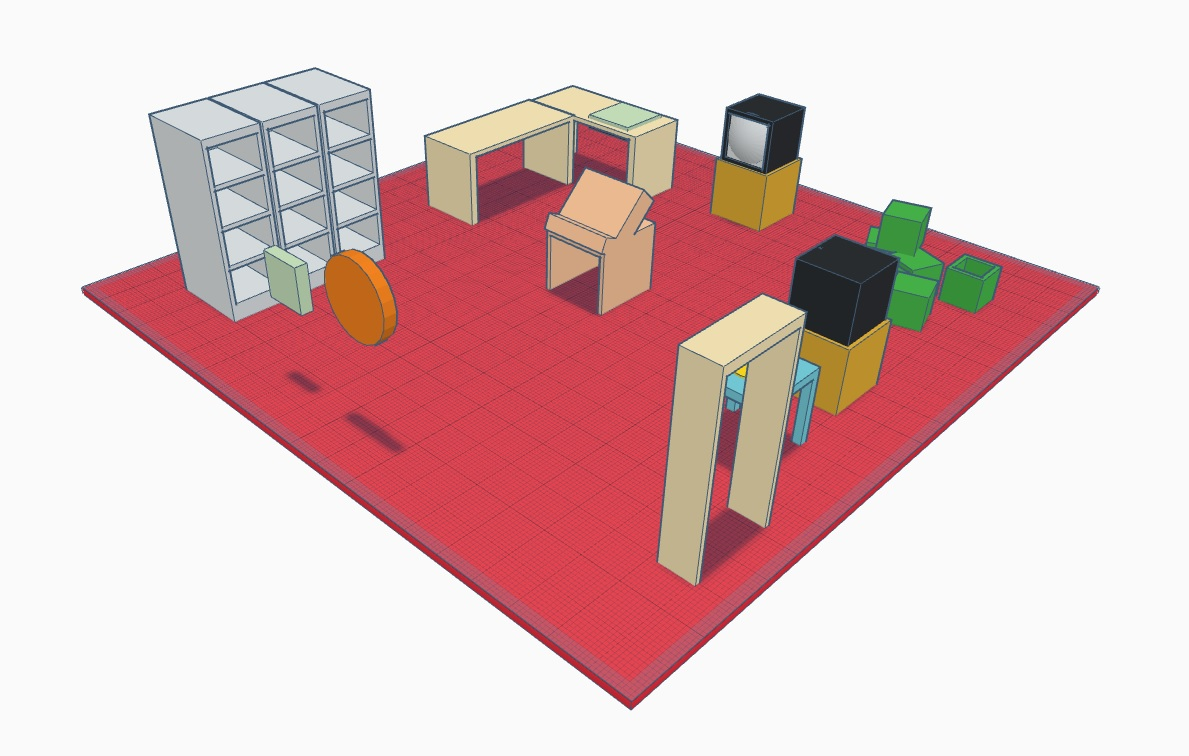
\includegraphics[width=0.90\columnwidth]{Images/EscapeRoomIsoFront.jpg}
    \caption{Front isometric scale depiction of the initial escape room layout.}
\end{figure}

\begin{figure}[ht]
    \centering
    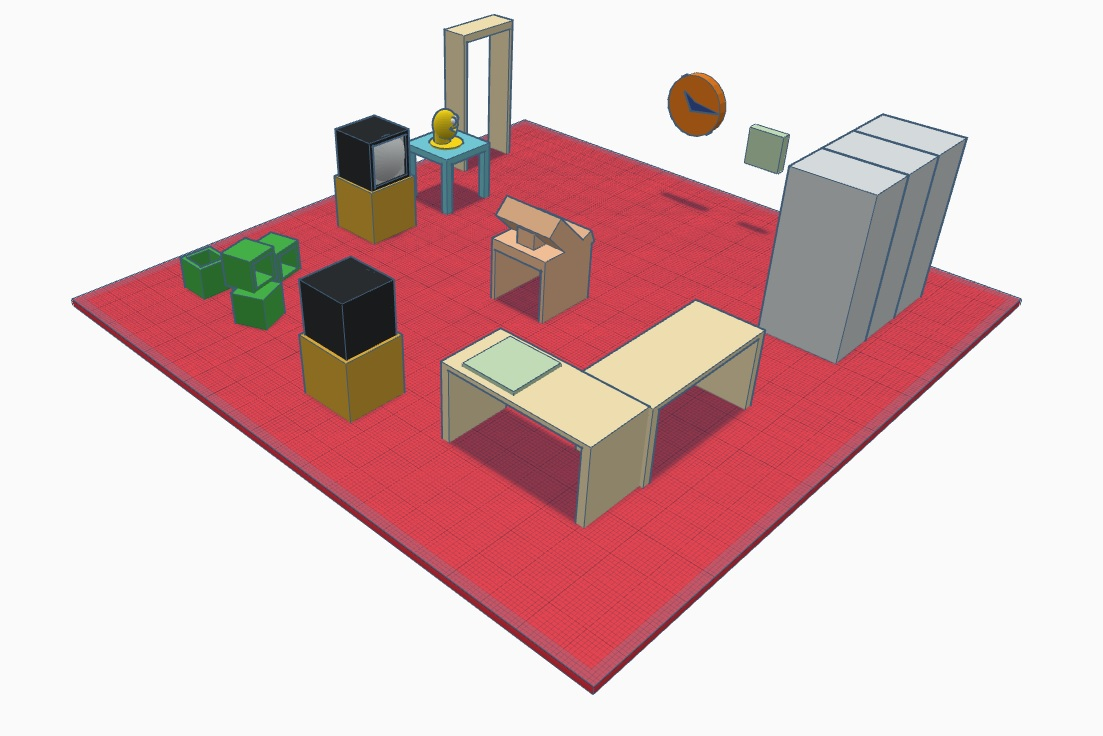
\includegraphics[width=0.75\columnwidth]{Images/EscapeRoomIsoRear.jpg}
    \caption{Rear isometric scale depiction of the initial escape room layout.}
\end{figure}

% *************************************************************************************************************************************
% ************************************* THIS SECTION MUST BE REVISED ******************************************************************
% *************************************************************************************************************************************
\section{Evaluation} % Kyle

\begin{figure}[H]
    \centering
    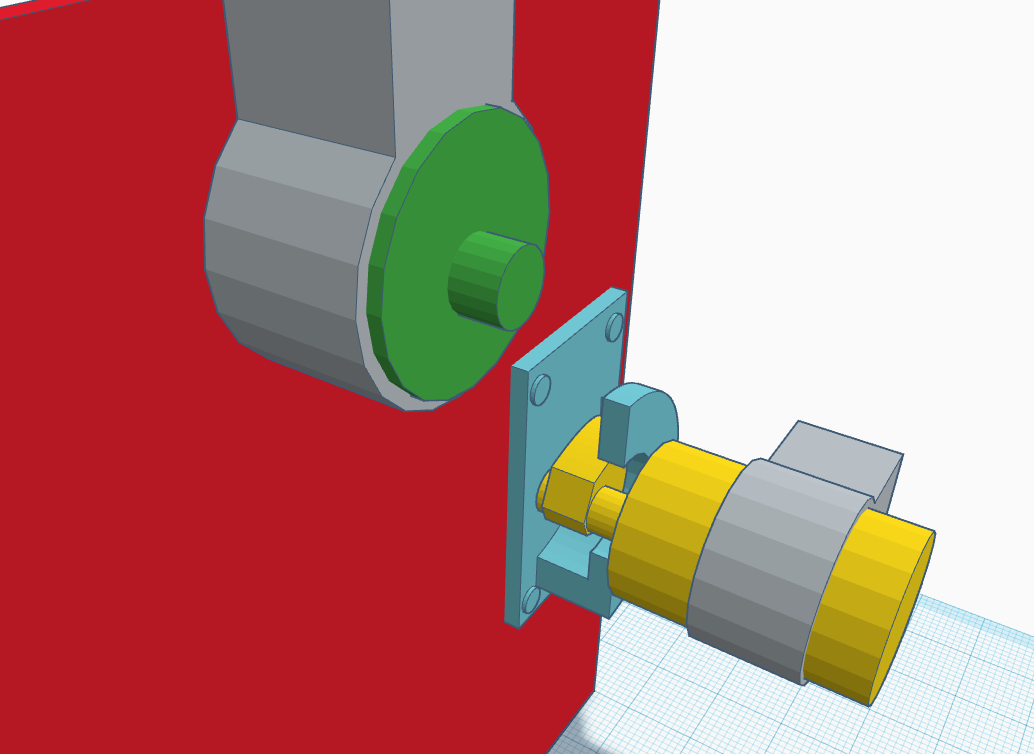
\includegraphics[width=0.85\columnwidth]{Images/ClosedLock.png}
    \caption{When the motor arms are under the metal plate, the container remains locked}
\end{figure}

\begin{figure}[H]
    \centering
    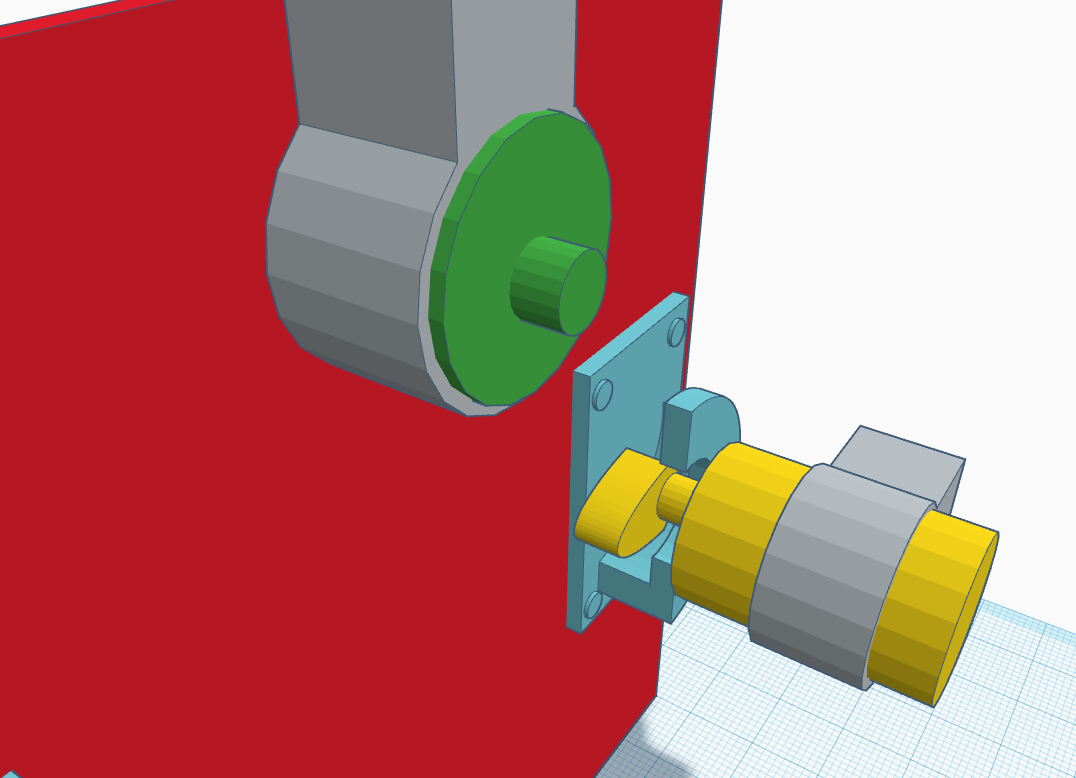
\includegraphics[width=0.85\columnwidth]{Images/OpenLock.png}
    \caption{When the arms are rotated out from the metal plate, the container is unlocked and can manually be opened.}
\end{figure}

\begin{figure}[H]
    \centering
    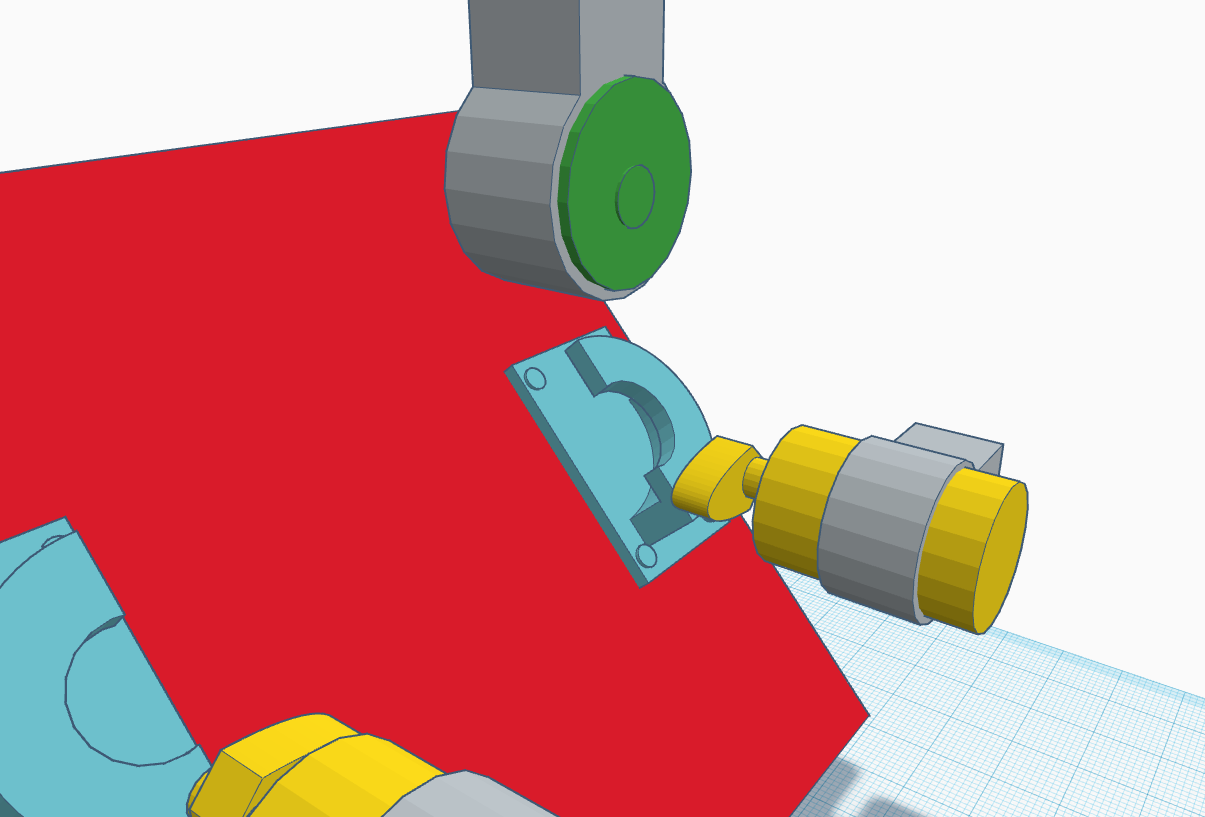
\includegraphics[width=0.85\columnwidth]{Images/OpenContainer.png}
    \caption{The internal solenoid can be used for several effects. For example, when facing the container opening, it can pop the
        door open automatically. If it is facing a wall, it will create a knock sound, or if it does not contact with anything, it can
        make a clicking noise to signal the box is unlocked.}
\end{figure}

\subsection*{Wi-Fi}
Wi-Fi will act as an incredibly reliable and secure option for our senior project. One of the benefits of Wi-Fi
is that is it so widely supported. There are lots of libraries that would make communication and connection over
Wi-Fi as simple as possible. Plus, the connection range is incredibly good over Wi-Fi, and the data rate is quite high
(around 54 Mbps)~\cite{wifiVsZigbee}. There are two drawbacks to Wi-Fi, however, the first being that it uses a bit more energy than Zigbee
to operate, which may become a problem depending on how many of our components need to operate on a portable energy
source. The second is that there are so many other devices that operate using Wi-Fi, and we may want the privacy that
a connection through Zigbee would provide.

\subsection*{Zigbee}
On the other hand, Zigbee would be an interesting option for a variety of reasons. The most beneficial reason to using
Zigbee would be its topology. Zigbee uses a mesh network topology, which allows each of the network devices to connect with
one another, rather than being dependent upon a central hub to manage the details of the escape room. This would decrease
the number of ``network-hops'' a command would need to traverse, allowing components to tell locks when their puzzle has been
solved. We may end up needing a central hub, so this benefit could nullified, but I digress. Furthermore, Zigbee is much less
widely used than Wi-Fi providing us with a unique experience when trying to get all of our components to communicate
with one another. It also consumes less energy and has a lower data transmission rate than Wi-Fi (maxing out at 250 Kbps),
which could help our wireless components be more energy efficient~\cite{wifiVsZigbee}. These details are yet to be explored,
however, and will need to be more properly considered when we have a more developed plan as to what our escape room is going to require.


%   ********************************************************************************************************
%   ********************* CONCLUSION TO BE COMPLETED TOGETHER **********************************************
%   ********************************************************************************************************
\section{Conclusions}
In conclusion, we are confident that this project will help us grow and become more capable
engineers in the future. We are going to learn more about how to deal with lots of interconnected
micro-systems, how to create a compelling and immersive story, how to properly document and track
our work, and how to work together as a team on a long-term development project. All of these things
are incredibly valuable to prospective employers, and we are excited to leave college as prepared
as possible to enter the workforce. Furthermore, this is a project that we are all incredibly excited
about, which will help us produce something that we can be proud of by the end of next semester!

\section{Appendix A: Reference Material}

\subsection{Bill of Materials}
In order to have a functioning project that we can be proud of, we are going to need a lot of materials.
A list of these materials have been included below
\begin{itemize}
    \item Programmable microcontrollers
    \item Analog clock
    \item Cameras
    \item Small CRT televisions
    \item Audio cassette player
    \item Writable audio cassette tapes
    \item MP3 digital audio controller
    \item Speakers
    \item Motors (To act as lock releases)
    \item Solenoids
    \item LED Display
    \item Adjustable RGB lights
    \item Wireless communication modules
    \item Storage containers
    \item Busts with detachable modules
\end{itemize}

\section{Appendix B: Troubles of note during development}

\begin{thebibliography}{00}

    \bibitem{wikipediaEscapeRoom} “Escape room,” Wikipedia, 10-Feb-2023. [Online]. Available: \url{https://en.wikipedia.org/wiki/Escape_room}. [Accessed: 24-Mar-2023].
    \bibitem{germanEscapeRoom} M. Pfeifer, B. Völker, S. Böttcher, S. Köhler, and P. M. Scholl, “Teaching embedded systems by constructing an escape room,” Proceedings of the 52nd ACM Technical Symposium on Computer Science Education, 2021.    
    \bibitem{whatIsAnEscapeRoom} A. Ascalon, “Escape rooms: Everything you need to know (2022),” Escape Rooms | Everything You Need To Know (2022), 01-Dec-2022. [Online]. Available:  \url{https://theescapegame.com/blog/what-is-an-escape-room/}. [Accessed: 24-Mar-2023].
    \bibitem{wifiVsZigbee} B. Priya, “What are the differences between Zigbee and Wi-Fi,” Tutorials Point, 17-Mar-2022. [Online]. Available: \url{https://www.tutorialspoint.com/what-are-the-differences-between-zigbee-and-wi-fi}. [Accessed: 03-May-2023].

\end{thebibliography}




\end{document}